\section{Effects on news' distribution among users}
Memory selects the amount of news can be remembered: this could affect news' distribution among users.
Indeed, if we insert in the network a certain number of news (i.e. launching a simulation with many news), they will reach a fraction of users (FOUR, fraction of users reached) at a fixed time.\\
News spreading over time, in general, starts with a fluctuating transient and then reaches a stationary state: from a ``microscopic'' point of view, users' identity might vary but the fraction is pretty much the same. \\
News spreading over time, in general, starts with a fluctuating transient and then reaches a stationary state: from a ``microscopic'' point of view, users' identity might vary but the fraction is pretty much the same.
It is statistically correct to compute, for every news, the average FOUR over time, with a certain threshold in order to neglect the transient ( the end time and the threshold are experimentally determined by free trials).
We obtain in this  way a distribution of average FOURs, one for each news.\\
Gini index measures the inequality of a distribution. Values of 0 and 1 stand for, respectively, the maximum homogeneity and the maximum heterogeneity.
However, this index is a function of random values: mean and error have to be estimated.\\
A certain number of samples is created by sampling with replacement of the average FOUR distribution: Gini index is computed for each one of them.
Now we have a population of Gini indexes, and we can extract mean and error: the whole process is known as bootstrap (see Appendix 1 for error estimation).\\
In practical terms, for every level of  memory, a simulation with twenty news is run out: Gini index' mean and error are computed like before.
The Gini index-memory plot shows a highly non-linear behaviour: sigmoid and gaussian seem to better represent data.\\
 In order to select the best-fit function, Chi-square is computed for both of them. \\
Because of asymmetric error bars, the optimization function is slightly different from the standard one, used for weighted interpolation: see Appendix 2 for more details.
Interpolation results are shown below:

%\begin{figure}[!h]
  %\centering
  %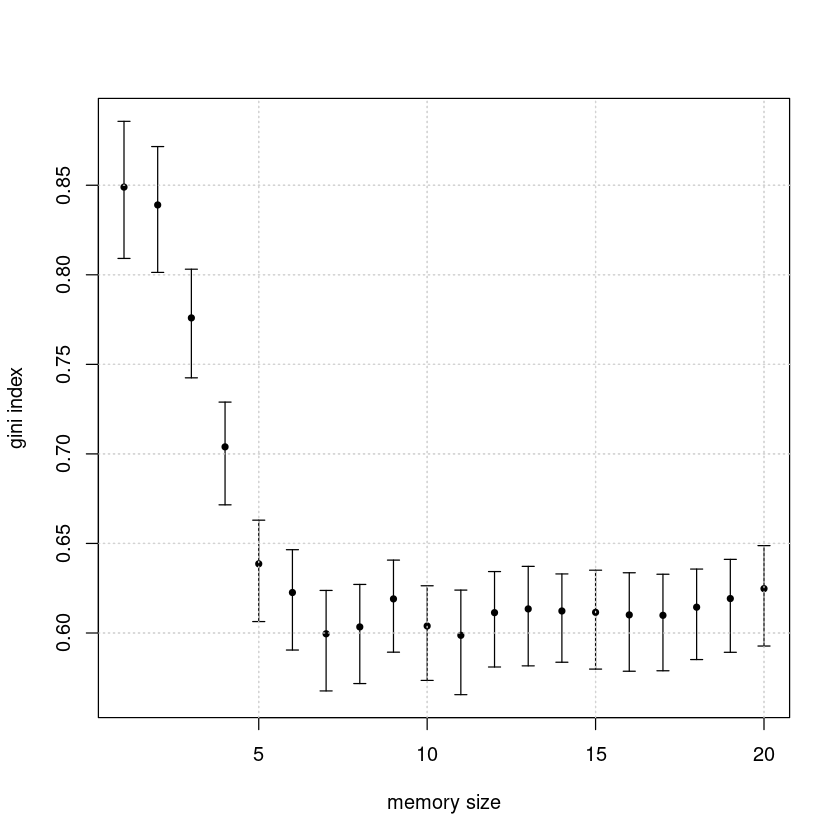
\includegraphics[width=.7\columnwidth]{img/gini_memory.png}
  %\caption{Gini index-memory plot with errorbars}
  %\label{fig:ginimem}
%\end{figure}

Risultati
subplot grafici??
manca grassetto/corsivo
immagini esplicative appendix2


\subsection{Appendix 1: errorbars for Gini index}

Bootstrap method is used to compute Gini index' mean and error: while for the former the process is pretty straigthforward, this is not the case for the latter.
Average FOUR distribution is asymmetrical and, in general, non-normal; we consider two different types of error.
Given N samples ${x_1,...,x_N}$ whose mean is $\mu$, correct standard deviation is:

$$
\sigma=\sqrt{\frac{\sum_{i=1}^{i=N}(x_i - \mu)^2}{N-1}}
$$


Quantile Standard Error (	QSE), instead, estimates the error by considering the fraction of samples falling within a certain interval: the whole distribution is divided in equal parts by a certain amount of ``quantiles''.\\
For example, in a Normal distribution, the interval $[\mu -\sigma, \mu +\sigma]$ ``covers'' approximately 68\% of the samples(figura...).
In ``quantiles'' terms (percentiles in this case), our errorbar starts from the $17^{th}$ percentile and ends in the $68^{th}$ percentile.\\
For non-normal distributions, standard deviation in general does not follow this property: to preserve it, we can compute QSE with the previous choice of quantiles, just by looking at the cumulative distribution, when values 0.17 and 0.68 are reached.

Immagini di gaussiana con 1 e 2 sigma e cumulativa della gaussiana...

The overall error is divided twofold, ``rightmost'' and ``leftmost''  the mean. For every part of the interval, we pick the ``largest'' between standard deviation and QSE: this conservative approach avoids underestimations in both directions.




\subsection{Appendix 2: asymmetric errorbars fitting}
The aim of a standard fitting problem is to find a function which reproduces experimental observations.
Let $f_{\theta}$ be the candidate function: $\theta=(\theta_1,...,\theta_m)$ is a vector of m parameters which completely determines function's values.
The optimization is performed with respect to $\theta$ parameters.\\
Given N datapoints with coordinates ${(x_i,y_i)}$ and y-errorbars $\sigma_i$, i=1,...,N, the usual optimization function for weighted interpolation is:

$$
E(\theta)= \sum_{i=1}^{N} \frac{(f_{\theta}(x_i)-y_i)^2}{\sigma_{i}^2}
$$


However, this formula is only applicable for gaussian errors, expressed by the standard deviation: in the problem we are facing, errorbars are not even symmetric.
We have developed an approximate optimization function which counts in this asymmetry.
In a weighted interpolation, the weight is the square inverse of the standard deviation: the ``shortest'' the errorbar, the closest will be $f(x_i)$ to $y_i$.
It might be an idea to split the error in two contributions, to be ``activated'' if the function value is greater or lower than the experimental value.
Let a and b be, respectively, the errorbars ``over'' and ``down'' the mean point: the optimization function for asymmetric errobars interpolation is:

$$
E= \sum_{i=1}^{N} \frac{(f(x_i)-y_i)^2}{a^{2}H(f(x_i)-y_i)+b^{2}H(y_i-f(x_i))}
$$

H(x) is the Heaviside function, which gives an ouput of 1 for $x>0$, 0 otherwise.\\
$f(x_i)$ ``sees'' an error of a if over $y_i$, or b if down.
The optimization is performed by specific R packages.
